\documentclass[10pt]{article}
\usepackage{icmlko}

\icmlmeta{IP 파운데이션 월드모델}{17}{시드가 결론을 삼킨다}{시드 스무 개로 재보니 공유 헤드의 우위가 잡음 안에 있었다 --- 그리고 단순한 쪽이 이긴다}

\begin{document}

\twocolumn[
\icmlheader

\begin{abstract}
노트 16은 신경망의 시드 분산이 크다는 것을 한계로 적고 정량화를 다음 과제로
남겼다. 시드 20개로 재봤다. \textbf{분산이 효과 크기를 삼킨다} --- 팝업에서
공유 헤드의 상수 대비 이득이 0.0149인데 시드 표준편차가 0.0783이다. 5.3배다.
게임은 이득이 음수이고(즉 상수보다 나쁘고) 표준편차가 0.0848이다. 이어서 노트 15가
남긴 마지막 반증 조건 --- 공유 헤드를 포기한 대조군 --- 을 돌렸다. 출처마다 따로
학습해 예측을 평균만 내면 \textbf{공유 헤드보다 낫고 분산도 절반이다}(게임
0.8454 대 0.7872, 표준편차 0.085 대 0.049). 공동 학습은 이득이 아니라 손해다.
그리고 세 방법 모두 \textbf{ridge 쌍 전이보다 나쁘다}(세 도메인 평균 0.6702 대 0.7244·0.7490).
결론은 노트 6이 이미 말한 것이다 --- \textbf{이 표본에서 신경망은 아직 이르다.}
노트 14를 완전히 철회하고, 파운데이션 구조를 ``측정된 축 $\to$ 선형 모델 $\to$
도메인 간 계수 전이''로 확정한다. 공유 표현 주장 자체는 살아 있다(노트 16의 전이
넷은 결정론적 ridge에서 나왔다). 무너진 것은 신경망 구현이다.
\end{abstract}
]

\section{시드를 스무 개 돌렸다}

노트 16의 한계 절에 이렇게 적었다.

\begin{quote}\fontsize{9.2}{11}\selectfont
신경망의 시드 분산이 크다. 같은 설정에서 팝업 예측 MAE가 시드 수에 따라 0.7357에서
0.7733까지 움직였다. \dots\ 보고한 파운데이션 수치는 이 분산 안에 있다.
\end{quote}

``분산 안에 있다''고 짐작만 하고 넘어갔다. 재봤다.

\begin{figure}[t]
\centering

\includegraphics[width=\textwidth]{figs/seed.pdf}
\caption{시드 20개, 평균 $\pm$1 표준편차. 가로줄이 상수와 ridge 쌍 전이다.
오차 막대가 두 가로줄 사이 거리보다 크다.}
\end{figure}

\begin{table}[t]
\centering\tsize
\caption{시드 20개 기준 평균절대오차.}
\begin{tabular}{lrrr}
\toprule
대상 & 상수 & 공유 헤드 & 출처별 앙상블 \\
\midrule
팝업   & 0.7596 & 0.7447 $\pm$ 0.0783 & 0.7440 $\pm$ 0.0506 \\
아이돌 & 0.6474 & 0.6568 $\pm$ 0.0419 & 0.6421 $\pm$ 0.0264 \\
게임   & 0.7701 & 0.8454 $\pm$ 0.0848 & 0.7872 $\pm$ 0.0486 \\
\bottomrule
\end{tabular}
\end{table}

\begin{figure}[t]
\centering
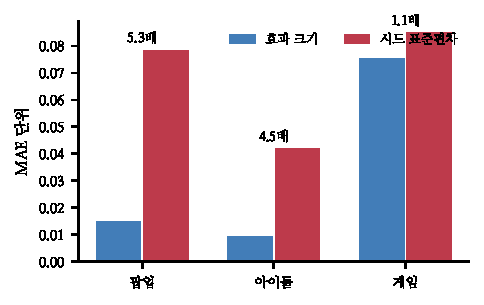
\includegraphics[width=\columnwidth]{figs/ratio.pdf}
\caption{효과 크기와 시드 표준편차의 비율. 잡음이 신호의 몇 배다.}
\end{figure}

팝업에서 공유 헤드는 상수를 0.0149 이긴다. 시드 표준편차는 0.0783이다.
\textbf{잡음이 신호의 5.3배다.} 시드 하나만 보고 ``이겼다''고 쓰면 동전을 한 번
던지고 결론을 내는 것과 같다.

\claimx{이 표본에서 신경망 결과는 시드 하나로 보고할 수 없다. 시드 분산이 상수
대비 효과 크기의 4--5배다(팝업 5.3배, 아이돌 4.5배). 게임은 효과가 음수라
비율 자체가 의미를 잃는다.}{표본이 커져 시드 표준편차가 효과 크기의 3분의 1 아래로
내려가면 단일 시드 보고가 가능해진다.}

\section{공유 헤드를 포기해 봤다}

노트 15는 공유 헤드가 쌍 전이보다 못한 이유를 계수 크기 차이로 지목하고 반증
조건을 적었다 --- 방향까지 도메인별로 풀었을 때(공유 헤드를 포기했을 때) 격차가
커지면 문제는 눈금이 아니라 공유 자체다.

대조군은 단순하다. 두 출처 도메인을 \emph{함께} 학습하지 않고 \emph{따로} 학습한
뒤 예측을 평균만 낸다. 공유되는 것이 없다.

\begin{table}[t]
\centering\tsize
\caption{공동 학습 대 단순 앙상블(시드 20개).}
\begin{tabular}{lrr}
\toprule
대상 & 공유 헤드 & 출처별 앙상블 \\
\midrule
팝업   & 0.7447 $\pm$ 0.078 & \textbf{0.7440} $\pm$ 0.051 \\
아이돌 & 0.6568 $\pm$ 0.042 & \textbf{0.6421} $\pm$ 0.026 \\
게임   & 0.8454 $\pm$ 0.085 & \textbf{0.7872} $\pm$ 0.049 \\
\bottomrule
\end{tabular}
\end{table}

세 대상 모두 앙상블이 낫고, 분산은 절반 수준이다. 게임에서는 격차가 0.058로 크다.

\claimx{공동 학습은 이득이 아니라 손해다. 출처마다 따로 학습해 예측을 평균만
내는 편이 세 대상 모두에서 낫고 분산도 절반이다.}{도메인 수가 늘어(다섯 이상)
공동 학습이 앙상블을 넘어서면, 이 결과는 출처가 둘뿐이라 생긴 것이다.}

이것은 노트 15가 세운 배율 가설의 마지막 반증이기도 하다. 문제는 계수 눈금이
아니라 \emph{공유 자체}였다. 출처가 둘뿐인 상태에서 하나의 헤드를 강요하면
두 도메인의 절충으로 끌려갈 뿐 얻는 것이 없다.

\section{그리고 셋 다 선형 모델보다 나쁘다}

\begin{figure}[t]
\centering

\includegraphics[width=\textwidth]{figs/ladder.pdf}
\caption{세 도메인 평균. 단순한 쪽이 이긴다.}
\end{figure}

\begin{table}[t]
\centering\tsize
\caption{세 도메인 평균 MAE.}
\begin{tabular}{lr}
\toprule
방법 & 평균 MAE \\
\midrule
ridge 쌍 전이 & \textbf{0.6702} \\
출처별 앙상블 (신경망) & 0.7244 \\
상수 & 0.7257 \\
공유 헤드 (신경망) & 0.7490 \\
\bottomrule
\end{tabular}
\end{table}

측정된 축을 ridge에 그대로 넣고 계수만 옮기는 것이 신경망 어느 구성보다 낫다.
공유 헤드는 상수보다도 나쁘다.

\claimx{노트 14를 완전히 철회한다. 파운데이션 구조의 신경망 구현은 이 표본에서
정당화되지 않으며, 측정된 축을 선형 모델에 넣고 계수를 옮기는 것이 모든
신경망 구성보다 낫다.}{표본이 도메인당 수백 건으로 커진 뒤 신경망이 ridge를
넘어서면 철회 사유는 구조가 아니라 표본이었던 것이다.}

\section{그러면 무엇이 남았나}

무너진 것과 남은 것을 분명히 갈라 둔다.

\paragraph{무너진 것 --- 신경망 구현}
앵커된 슬롯, 도메인별 인코더, 공유 선형 헤드. 노트 5--7이 제약을 좁혀 만든
구조인데, 그 제약들은 \emph{팝업 단일 도메인}에서 도출됐고 표본이 75건이었다.
세 도메인으로 넓히자 시드 분산이 결과를 삼켰다.

\paragraph{남은 것 --- 공유 표현 주장}
노트 16이 보고한 전이 넷은 전부 \emph{결정론적} ridge에서 나왔다. 시드가 없으므로
이 결과들은 이 노트의 비판을 받지 않는다.

\begin{itemize}[leftmargin=1.1em,itemsep=0.15em]
\item 팝업 $\to$ 아이돌 p=0.0013
\item 게임 $\to$ 아이돌 p$<$0.0001
\item 아이돌 $\to$ 팝업 p=0.0480
\item 게임 $\to$ 팝업 p=0.0003
\end{itemize}

두 축(타깃 폭, 굿즈 규모)이 세 도메인에서 같은 부호로 작동하고 계수가 옮겨진다는
사실은 그대로다.

\paragraph{그래서 확정 구조}
\begin{quote}\fontsize{9.5}{11.5}\selectfont
도메인마다 축을 \textbf{측정}하고, 축에서 결과로 가는 \textbf{선형} 관계를 한
도메인에서 추정해 다른 도메인에 옮긴다. 인코더도 공동 학습도 현재 표본에서는
불필요하다.
\end{quote}

이것은 노트 6이 이미 말한 것이다 --- ``n=75에서 신경망은 아직 이르다.'' 그것을
확립해 놓고 노트 14에서 다시 신경망을 지었다. 도메인이 셋이 됐으니 괜찮을 것이라
가정했는데, 도메인이 늘어도 도메인당 표본은 그대로였다.

\section{한계}

\begin{itemize}[leftmargin=1.1em,itemsep=0.15em]
\item 시드 20개는 표준편차 추정에 충분하지만 평균 추정에는 넉넉하지 않다.
      보고한 평균 자체가 $\pm$0.02 정도 흔들린다.
\item 신경망 하이퍼파라미터(층 폭 16, 드롭아웃 0.15, 앵커 8.0)를 조율하지 않았다.
      조율하면 분산이 줄 수 있으나, 조율에 쓸 검증 표본이 없다.
\item ridge 쌍 전이의 ``최선''은 사후 선택이므로 신탁이다. 평균 쌍 전이와 비교하면
      격차가 줄어든다.
\item 앙상블은 출처 둘의 단순 평균이다. 가중을 배우면 라벨이 필요해진다.
\end{itemize}

\section{다음}

\begin{enumerate}[leftmargin=1.3em,itemsep=0.15em]
\item 입장 허들의 진짜 측정 --- 게임의 최소 사양 요구, 지역 제한 등 가격과
      분리된 접근 난이도.
\item 팝업·아이돌 굿즈 축의 누출 검정 --- 게임에서 쓴 30일 창 방식을 옮긴다.
\item 네 번째 도메인 --- 공동 학습이 앙상블을 넘어서려면 출처가 더 필요하다.
\item 도메인당 표본 확대 --- 신경망 재도전의 전제 조건.
\end{enumerate}

\vspace{0.6em}
\hrule height 0.3pt
\vspace{0.5em}
{\footnotesize
\textbf{참고문헌}\\[0.3em]
Bouthillier, X. et al. (2021). Accounting for variance in machine learning
benchmarks. \emph{MLSys 2021}.\\[0.15em]
Dietterich, T. G. (2000). Ensemble methods in machine learning.
\emph{Multiple Classifier Systems}, 1--15.\\[0.15em]
Grinsztajn, L., Oyallon, E., Varoquaux, G. (2022). Why do tree-based models still
outperform deep learning on typical tabular data? \emph{NeurIPS 2022}.\\[0.15em]
Standley, T. et al. (2020). Which tasks should be learned together in multi-task
learning? \emph{ICML 2020}, 9120--9132.
}

\end{document}
